\documentclass[11pt]{amsart}
\usepackage{geometry}                % See geometry.pdf to learn the layout options. There are lots.
\geometry{letterpaper}                   % ... or a4paper or a5paper or ... 
%\geometry{landscape}                % Activate for for rotated page geometry
%\usepackage[parfill]{parskip}    % Activate to begin paragraphs with an empty line rather than an indent
\usepackage{graphicx}
\usepackage{amssymb}
\usepackage{amsmath}
\usepackage{epstopdf}
\usepackage[linesnumbered,vlined,algoruled]{algorithm2e}
\usepackage{url}
\usepackage{mathtools}
\DeclarePairedDelimiter{\ceil}{\lceil}{\rceil}
\DeclarePairedDelimiter{\floor}{\lfloor}{\rfloor}
\DeclareGraphicsRule{.tif}{png}{.png}{`convert #1 `dirname #1`/`basename #1 .tif`.png}
\DeclareMathOperator*{\argmax}{arg\,max}
\DeclareMathOperator{\argmin}{arg\,min}

\title{Computing Accurate Quantiles Using 1-D Clustering}
\author{Ted Dunning}
\email{ted.dunning@gmail.com}
\date{}                                           % Activate to display a given date or no date
\begin{document}
\begin{abstract}
An on-line algorithm for computing approximations of rank-based statistics is presented that allows controllable accuracy.  Moreover, this new algorithm can be used to compute hybrid statistics such as trimmed means in additional to computing arbitrary quantiles.  An unusual property of the method is that it allows a quantile $q$ to be computed with an accuracy relative to $q (1-q)$ rather than with an absolute accuracy as with most methods.  This new algorithm is robust with respect to highly skewed distributions or highly ordered datasets and allows separately computed summaries to be combined with no loss in accuracy.

An open-source implementation of this algorithm from the author.
\end{abstract}
\maketitle
\section{Introduction}
Given a sequence of numbers, it is often desirable to compute rank-based statistics such as the median, 95-th percentile or trimmed means in an on-line fashion, keeping only a small data structure in memory.  Traditionally, such statistics were often computed by sorting all of the data and then either finding the quantile of interest by interpolation or by processing all samples within particular quantiles.  This sorting approach is infeasible for very large datasets which has led to interest in on-line approximate algorithms.

One early algorithm for computing on-line quantiles is described in \cite{Chen2000}.  In that work specific quantiles were computed by incrementing or decrementing an estimate by a value proportional to the simultaneously estimated probability density at the desired quantile.  This method is plagued by a circularity in that estimating density is only possible by estimating yet more quantiles.  Moreover, this work did not allow the computation of hybrid quantities such as trimmed means.

An alternative approach is described in \cite{qdigest}.  In this work, incoming values are assumed to be integers of fixed size. Such integers can trivially be arranged in a perfectly balanced binary tree where the leaves correspond to the integers and the interior nodes correspond to bit-wise prefixes. This tree forms the basis of the data structure known as a Q-digest.  The idea behind a Q-digest is that in the uncompressed case, counts for various values are assigned to leaves of the tree.  To compress this tree, sub-trees are collapsed and counts from the leaves are aggregated into a single node representing the sub-tree such that the maximum count for any collapsed sub-tree is less than a threshold that is a small fraction of the total number of integers seen so far.  Any quantile can be computed by traversing the tree in left prefix order, adding up counts until the desired fraction of the total is reached.  At that point, count for the last sub-tree traversed can be used to interpolate to the desired quantile within a small and controllable error.  The error is bounded because the count for each collapsed sub-tree is bounded.

The two problems with the Q-digest are that it depends on the tree structure being known ahead of time and that the error bounds do not necessarily apply if the algorithm is used in an on-line fashion.  Adapting the Q-digest to use an balanced tree over arbitrary elements is difficult.  This difficulty arises because rebalancing the tree involves sub-tree rotations and these rotations may require reapportionment of previously collapsed counts in complex ways.  This reapportionment could have substantial effects on the accuracy of the algorithm and in any case make the implementation much more complex because the concerns of counting cannot be separated from the concerns of maintaining a balanced tree.  Another problem with Q-digests is that if they are subjected to compression during building, it isn't entirely clear how to handle compressed counts that move high above the leaves, but which eventually have non-trivial counts at a lower level in the tree.  The proof of correctness for Q-digests ignores this complication by only considering the case where counts are compressed after being collected on the leaves.  It would be desirable to have error bounds that apply to a completely on-line data structure.  These limitations do not apply in the original formulation of the Q-digest as a compression algorithm for quantile information, but current trends towards the use of on-line algorithms make these limitations awkward.

The work described here shows how the fundamental idea of a Q-digest can be easily extended to values in $\mathbb R$ without the complexity of apportioning counts during tree rebalancing.  Indeed, this new data structure eliminates the idea of a tree for storing the original samples, maintaining only the concept of collapsing groups of observations in a way that preserves accuracy.  This new algorithm, known as $1-d$ clustering, has well-defined and easily proven error bounds and allows parallel on-line operation.  A particularly novel aspect of the variant of $1-d$ clustering described here is that accuracy for estimating the $q$ quantile is relative to $q(1-q)$.  This is in contrast to earlier algorithms which had errors independent of $q$.  The relative error bound of $1-d$ cluster is convenient when computing quantiles for very small $q$ or for $q$ near $1$.  As with the Q-digest algorithm, the accuracy/size trade-off can be controlled by setting a single compression parameter.

The accuracy bounds are tight regardless of data ordering for the non-parallel on-line case.  In the case of parallel execution, the error bound is somewhere between the constant error bound and the relative error bound applies except in the case of highly ordered input data.  

\section{The Algorithm}
The basic outline of the algorithm for $1-d$ clustering is quite simple.  An initially empty ordered list of centroids, $C = [ c_1 \ldots c_m ]$ is kept.  Each centroid consists of a mean and a count.  To add a new value $x_n$ with a weight $w_n$, the set of centroids is found that have minimum distance to $x_n$.  This set is reduced by retaining only centroids with a count less than $4\delta q (1-q) n $ where $\delta$ controls the accuracy of quantile estimates and $q$ is the estimated quantile for the mean of the centroid.  If more than one centroid remains, one is selected at random.  If a centroid is found, then $(x_n,w_n)$ is added to that centroid.  It may happen that the weight $w_n$ is larger than can be added to the selected centroid.  If so, as much weight as possible is allocated to the selected centroid and the selection is repeated with the remaining weight.  If no satisfactory centroid is found or if there is additional weight to be added after all centroids with minimum distance are considered, then $x_n$ is used to form a new centroid and the next point is considered.  This procedure is shown more formally as Algorithm \ref{alg:full}.
 \begin{algorithm}[tb]
\SetKw{KwTo}{in}\SetKwFor{For}{for}{\string:}{}
\SetKwIF{If}{ElseIf}{Else}{if}{:}{elif}{else:}{}
\SetKwFor{While}{while}{:}{fintq}
\SetKwFor{For}{for}{\string:}{}
 \label{alg:full}
\SetNoFillComment
\KwIn{Ordered set of weighted centroids $C = \lbrace \rbrace$, sequence of real-valued, weighted points $X = \lbrace (x_1, w_1),\ldots (x_N, w_N)\rbrace$, and accuracy tolerance $\delta$}
\KwOut{final set $C=[c_1 \ldots c_m]$ of weighted centroids} 
\For{$(x_n, w_n) \in X$} {
  $z = \min | c_i.\mathtt{mean} - x |$\;
  $S = \lbrace c_i  :  |c_i.\mathtt{mean} - x| = z \wedge c_i.\mathtt{count} + 1 \le 4n\delta q(c_i) (1-q(c_i)) \rbrace $\;
   \While {$S \ne \lbrace \rbrace\wedge w_n > 0$} {
       Sample $c_j \sim \mathrm{Uniform}( S)$\;
       $\Delta w = \min(4n\delta q(c_i) (1-q(c_i))-c_j.\mathtt{count}, w_n)$\;
       $c_j.\mathtt{count} \gets c_j.\mathtt{count} + \Delta w$\;
       $c_j.\mathtt{mean} \gets c_j.\mathtt{mean} + \Delta w (x_n - c_j.\mathtt{mean})/c_j.\mathtt{count}$\;
       $w_n \gets w_n - \Delta w$\;
       $S \gets S - c_j$
     } 
     \If {$w_n > 0$} {
        $C \gets C + (x_n, w_n)$\;
      }
      \If {$|C| > K/\delta$} {
         $C \gets \mathtt{cluster}(\mathtt{permute}( C )) $\;
       }
} 
$C \gets \mathtt{cluster}(\mathtt{permute}( C )) $\;
\Return $ C $\\
\caption{$1-d$ Clustering}
\end{algorithm}

In this algorithm, a centroid object contains a mean and and a count.  Updating such an object with a new data-point $(x,w)$ is done using Welford's method \cite{wiki:welford, knuth2welford, welford62}.

The number of points assigned to each centroid is limited to $\max(1, \floor{4N\delta q(1-q})$ where $q$ is the quantile for the approximate mean of the centroid and $\delta$ is a parameter chosen to limit the number of points that can be assigned to a centroid.  Typically, this compression factor is described in terms of its inverse, $1/\delta$ in order to stay compatible with the conventions used in the Q-Digest.  The algorithm approximates $q$ for centroid $c_i$ by summing the weights for all of the centroids ordered before $c_i$:

\[q(c_i)=\frac{c_i.\mathtt{count}/2 + \sum_{j<i}c_j.\mathtt{count}} {\sum_j c_j.\mathtt{count}}\]

For centroids with identical means, order of creation is used as a tie-breaker to allow an unambiguous ordering.  In order to compute this sum quickly, the centroids can be stored in a data structure such as a balanced binary tree that keeps sums of each sub-tree.  Figure \ref{fig:gamma-sizes} shows actual centroid weights from multiple runs of this algorithm and for multiple distributions plotted against the ideal bound.

The use of a bound on centroid size that becomes small for extreme values of $q$ is useful because it allows relative error to be bounded very tightly, but may be problematic for some inputs.  If the values of $X$ are in ascending or descending order, then $C$ will contain as many elements as values that have been observed.  This will happen because each new value of $X$ will always form a new centroid because $q(1-q)\approx0$.  To avoid this pathology, if the number of centroids becomes excessive, the set of centroids is collapsed by recursively applying $1-d$ clustering to the centroids themselves after randomizing the order of the centroids.  

After passing through all of the data points, the centroids are recursively clustered one additional time.  This allows adjacent centroids to be merged if they do not violate the size bound.  This final pass typically reduces the number of centroids by 20-40\% with no apparent change in accuracy.

Initial versions of this algorithm tried to use the centroid index $i$ as a surrogate for $q$, applying a correction to account for the fact that extreme centroids have less weight.  Unfortunately, it was difficult to account for the fact that the distribution of centroid weights changes during the course of running the algorithm.  Initially all weights are $1$.  Later, some weights become substantially larger.  This means that the relationship between $i$ and $q$ changes from completely linear to highly non-linear in a stochastic way.  This made it difficult to avoid too large or too small cutoff for centroids resulting in either too many centroids or poor accuracy.
\begin{figure}[htb] %  figure placement: here, top, bottom, or page
   \centering
   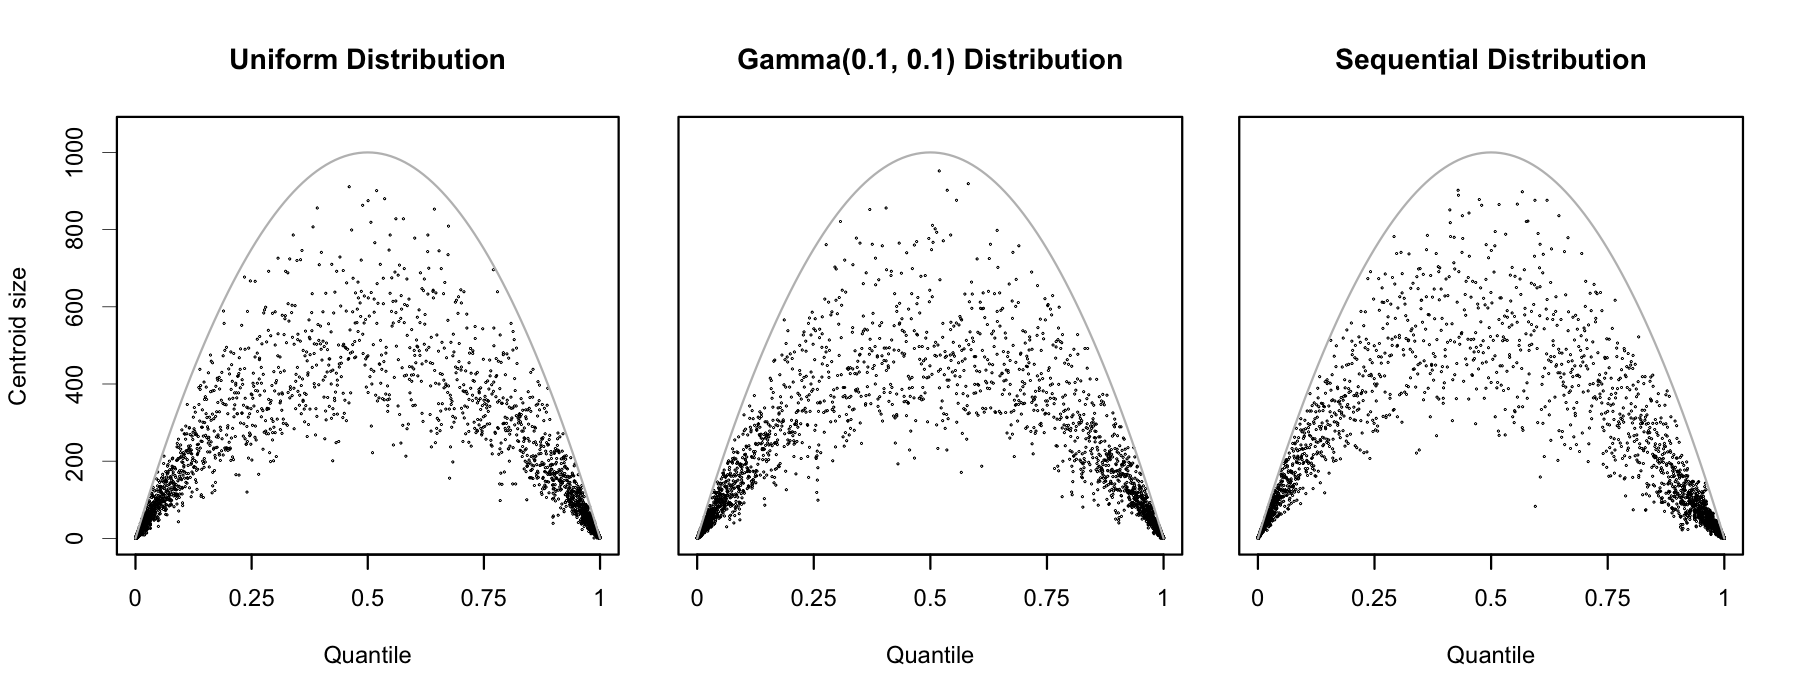
\includegraphics[width=6in]{sizes.png} 
   \caption{The accuracy of the size limit approximation used in the $1-d$ clustering algorithm.  The solid grey line indicates the size limit.  These diagrams also shows actual centroid weights for 5 test runs on $100,000$ samples from a uniform, $\Gamma(0.1, 0.1)$ and sequential uniform distribution.  In spite of the underlying distribution being skewed by roughly $30$ orders of magnitude of difference in probability density for the $\Gamma$ distribution, the centroid weight distribution is bounded and symmetric 
 as intended.  For the sequential uniform case, values are produced in sequential order with three passes through the $[0,1]$ interval with no repeated values.  As can be seen, this sequential presentation results in only a small asymmetry in the resulting size distribution.}
   \label{fig:gamma-sizes}
\end{figure}

The key property of this algorithm is that the final list of centroids $C$ is very close to what would have been obtained by simply sorting and then grouping adjacent values in $X$ into groups with the desired size bounds.  Clearly, such groups could be used to compute all of the rank statistics of interest here and if there are bounds on the sizes of the groups, then we have comparable bounds on the accuracy of the rank statistics in question.

That this algorithm does produce such an approximation is more difficult to prove rigorously, but an empirical examination is enlightening.  Figure \ref{fig:deviation} shows the deviation of samples assigned to centroids for uniform and highly skewed distributions.  These deviations are normalized by the half the distance between the adjacent two centroids.
\begin{figure}[htb] %  figure placement: here, top, bottom, or page
   \centering
   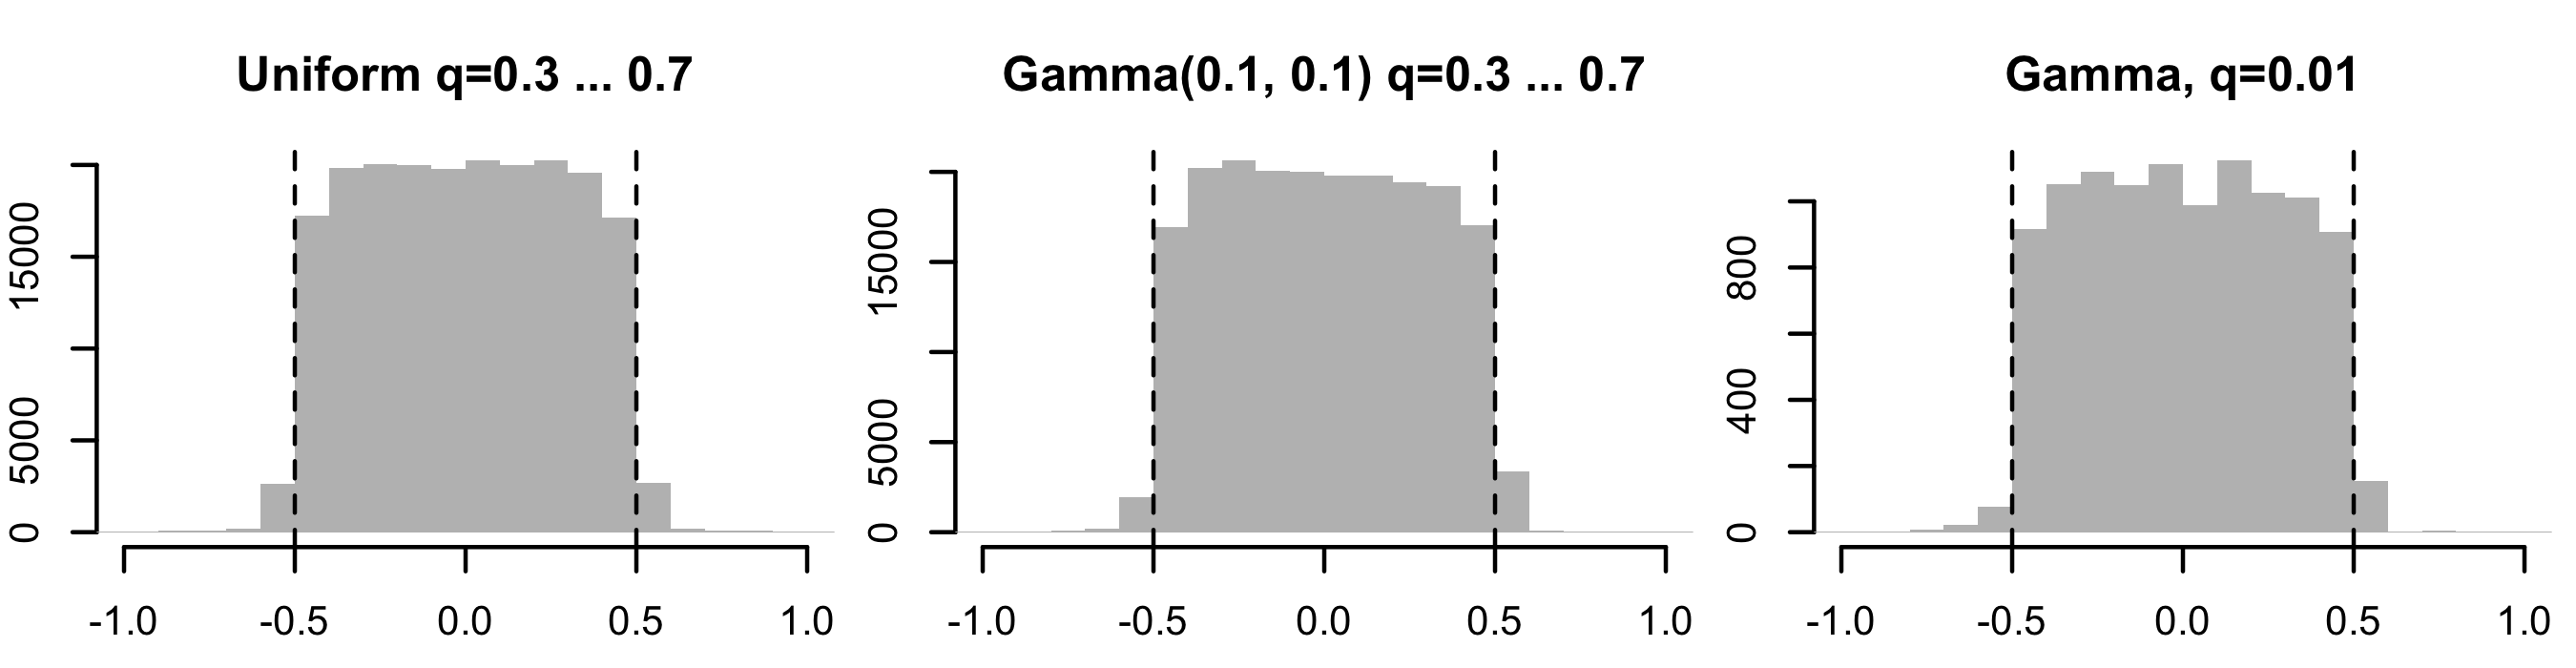
\includegraphics[width=4.5in]{deviation.png} 
   \caption{The deviation of samples assigned to a single centroid.  The horizontal axis is scaled to the distance to the adjacent centroid so a value of 0.5 is half-way between the two centroids. There are two significant observations to be had here.  The first is that relatively few points are assigned to a centroid that are beyond the midpoint to the next cluster.  This bears on the accuracy of this algorithm.  The second observation is that samples are distributed relatively uniformly between the boundaries of the cell.  This affects the interpolation method to be chosen when working with quantiles. The three graphs show, respectively, centroids from $q \in [0.3, 0.7]$ from a uniform distribution, centroids from the same range of a highly skewed $\Gamma(0.1, 0.1)$ and centroids from $q \in [0.01, 0.015]$ in a $\Gamma(0.1, 0.1)$ distribution.  This last range is in a region where skew on the order of $10^{22}$ is found. }
   \label{fig:deviation}
\end{figure}
This relatively uniform distribution for deviations among the samples assigned to a centroid is found for uniformly distributed samples as well as for extremely skewed data.  For instance, the $\Gamma(0.1, 0.1)$ distribution has a $0.01$ quantile of $6.07 \times 10^{-20}$, a median of $0.006$ and a mean of $1$.  This means that the distribution is very skewed.  In spite of this, samples assigned to centroids near the first percentile are not noticeably skewed within the centroid.  The impact of this uniform distribution is that linear interpolation allows accuracy considerably better than $q(1-q)/\delta$.

\subsection{Finding the cumulative distribution at a point}
Algorithm \ref{alg:quantile} shows how to compute the cumulative distribution $P(x)=\int_{-\infty}^x p(\alpha) \, d\alpha$ for a given value of $x$ by summing the contribution of uniform distributions centered at each the centroids.  Each of the centroids is assumed to extend symmetrically around the mean for half the distance to the adjacent centroid.

 \begin{algorithm}[b]
 \label{alg:quantile}
\SetKw{KwTo}{in}\SetKwFor{For}{for}{\string:}{}
\SetKwIF{If}{ElseIf}{Else}{if}{:}{elif}{else:}{}
\SetKwFor{While}{while}{:}{fintq}
\SetKwFor{For}{for}{\string:}{}
\SetNoFillComment
\KwIn{Centroids derived from distribution $p(x)$, $C = [ \ldots [m_i, s_i, k_i] \ldots ]$ , value $x$ }
\KwOut{Estimated value of $q = \int_{-\infty}^x p(\alpha) d \alpha$} 
$t = 0$, $N = \sum_i k_i$\;
\For {$i \in 1\ldots m$} {
    \uIf {$i < m$} {
      $\Delta \gets (c_{i+1}.\mathtt{mean} - c_i.\mathtt{mean})/2$\;
    } \Else {
      $\Delta \gets (c_{i}.\mathtt{mean} - c_{i-1}.\mathtt{mean})/2$\;
    }
    $z = \max(-1, (x-m_i)/\Delta)$\;
  \If {$z < 1$} {
    \Return $(t + \frac{k_i} N \frac{z+1} {2})$
  }
  $t \gets t + k_i$\;
}
\Return $1$
\caption{Estimate quantile $C.\mathtt{quantile}(x)$}
\end{algorithm}

For all centroids except one, this contribution will be either $0$ or $c_i.\mathtt{count}/N$ and the one centroid which straddles the desired value of $x$ will have a {\em pro rata} contribution somewhere between $0$ and $c_i.\mathtt{count}/N$. Moreover, since each centroid has count at most $\delta N$ the accuracy of $q$ should be accurate on a scale of $\delta$.  Typically, the accuracy will be even better due to the interpolation scheme used in the algorithm and because the largest centroids are only for values of $q$ near $0.5$.

The empirical justification for using a uniform distribution for each centroid can be seen by referring to again to Figure \ref{fig:deviation}.  
\subsection{Inverting the cumulative distribution}
Computing an approximation of the $q$ quantile of the data points seen so far can be done by ordering the centroids by ascending mean.  The running sum of the centroid counts will range from $0$ to $N=\sum c_i.\mathtt{count}$.  One particular centroid will have a count that straddles the desired quantile $q$ and interpolation can be used to estimate a value of $x$.  This is shown in Algorithm \ref{alg:estimate-quantile}.   Note that at the extreme ends of the distribution as observed, each centroid will represent a single sample so maximum resolution in $q$ will be retained.

 \begin{algorithm}[b]
 \label{alg:estimate-quantile}
\SetKw{KwTo}{in}\SetKwFor{For}{for}{\string:}{}
\SetKwIF{If}{ElseIf}{Else}{if}{:}{elif}{else:}{}
\SetKwFor{While}{while}{:}{fintq}
\SetKwFor{For}{for}{\string:}{}
\SetNoFillComment
\KwIn{Centroids derived from distribution $p(x)$, $C = [c_1 \ldots c_m ]$ , value $q$}
\KwOut{Estimated value $x$ such that $q = \int_{-\infty}^x p(\alpha) d \alpha$} 
$t = 0$, $q \gets q \sum c_i.\mathtt{count}$\;
\For {$i \in 1\ldots m$} {
  $k_i = c_i.\mathtt{count}$\;
  \If {$q < k_i$} {
    \uIf {$i = 1$} {
      $\Delta \gets (c_{i+1}.\mathtt{mean} - c_i.\mathtt{mean})$\;
    } \uElseIf {$i = m$} {
      $\Delta \gets (c_{i}.\mathtt{mean} - c_{i-1}.\mathtt{mean})$\;
    } \Else {
      $\Delta \gets (c_{i+1}.\mathtt{mean} - c_{i-1}.\mathtt{mean})/2$\;
    }
    \Return $m_i + \left( \frac {q-t} {k_i} - \frac 1 2 \right) \Delta$
  } 
  $t \gets t + k_i$
}
\Return $ c_m.\mathtt{mean}$
\caption{Estimate value at given quantile $C.\mathtt{icdf}(q)$}
\end{algorithm}

\subsection{Computing the trimmed mean}
The trimmed mean of $X$ for the quantile range $Q = [q_0,q_1]$ can be computed by computing a weighted average of the means of centroids that have quantiles in $Q$.  For centroids at the edge of $Q$, a {\em pro rata} weight is used that is based on an interpolated estimate of the fraction of the centroid's samples that are in $Q$.  This method is shown as Algorithm \ref {alg:estimate-trimmed-mean}.

 \begin{algorithm}[b]
 \label{alg:estimate-trimmed-mean}
\SetKw{KwTo}{in}\SetKwFor{For}{for}{\string:}{}
\SetKwIF{If}{ElseIf}{Else}{if}{:}{elif}{else:}{}
\SetKwFor{While}{while}{:}{fintq}
\SetKwFor{For}{for}{\string:}{}
\SetNoFillComment
\KwIn{Centroids derived from distribution $p(x)$, $C = [ \ldots [m_i, s_i, k_i] \ldots ]$ , limit values $q_0, q_2$}
\KwOut{Estimate of mean of values $x \in [q_0, q_1]$} 
$s = 0$, $k = 0$\;
$t = 0$, $q_1 \gets q_1 \sum k_i$, $q_1 \gets q_1 \sum k_i$\;
\For {$i \in 1\ldots m$} {
  $k_i = c_i.\mathtt{count}$\;
  \uIf {$q_1 < t+k_i$} {
    \uIf {$i > 1$} {
      $\Delta \gets (c_{i+1}.\mathtt{mean} - c_{i-1}.\mathtt{mean})/2$\;
    } \uElseIf {$i < m$} {
      $\Delta \gets (c_{i+1}.\mathtt{mean} - c_i.\mathtt{mean})$\;
    } \Else {
      $\Delta \gets (c_{i}.\mathtt{mean} - c_{i-1}.\mathtt{mean})$\;
    }
    $\eta = \left( \frac {q-t} {k_i} - \frac 1 2 \right) \Delta$\;
    $s \gets s + \eta \,k_i \,c_i.\mathtt{mean}$\;
    $k \gets k + \eta \,k_i$\;
  } 
  \uIf {$q_2 < t+k_i$} {
    \uIf {$i > 1$} {
      $\Delta \gets (c_{i+1}.\mathtt{mean} - c_{i-1}.\mathtt{mean})/2$\;
    } \uElseIf {$i < m$} {
      $\Delta \gets (c_{i+1}.\mathtt{mean} - c_i.\mathtt{mean})$\;
    } \Else {
      $\Delta \gets (c_{i}.\mathtt{mean} - c_{i-1}.\mathtt{mean})$\;
    }
    $\eta = \left(\frac 1 2 - \frac {q-t} { k_i}  \right) \Delta$\;
    $s \gets s - \eta \,k_i \,c_i.\mathtt{mean}$\;
    $k \gets k - \eta \,k_i$\;
  } 
  $t \gets t + k_i$
}
\Return $s/k$
\caption{Estimate trimmed mean.  Note how centroids at the boundary are included on a {\em pro rata} basis.}
\end{algorithm}
\section{Empirical Assessment}
\subsection{Accuracy of estimation for uniform and skewed distributions}
Figure \ref{fig:uniform-error} shows the error levels achieved with $1-d$ clustering in estimating quantiles of 100,000 samples from a uniform and from a skewed distribution.  In these experiments $\delta=0.01$ was used since it provides a good compromise between accuracy and space.  There is no visible difference in accuracy between the two underlying distributions in spite of the fact that the underlying densities differ by more roughly 30 orders of magnitude.  The accuracy shown here is computed by comparing the computed quantiles to the actual empirical quantiles for the sample used for testing and is shown in terms of $q$ rather than the underlying sample value.  At extreme values of $q$, the actual samples are preserved as centroids with weight $1$ so the observed for these extreme values is zero relative to the original data.  For the data shown here, at $q=0.001$, the maximum weight on a centroid is just above $4$ and centroids in this range have all possible weights from $1$ to $4$.  Errors are limited to, not surprisingly, just a few parts per million or less.  For more extreme quantiles, the centroids will have fewer samples and the results will typically be exact.
\begin{figure}[htb] %  figure placement: here, top, bottom, or page
   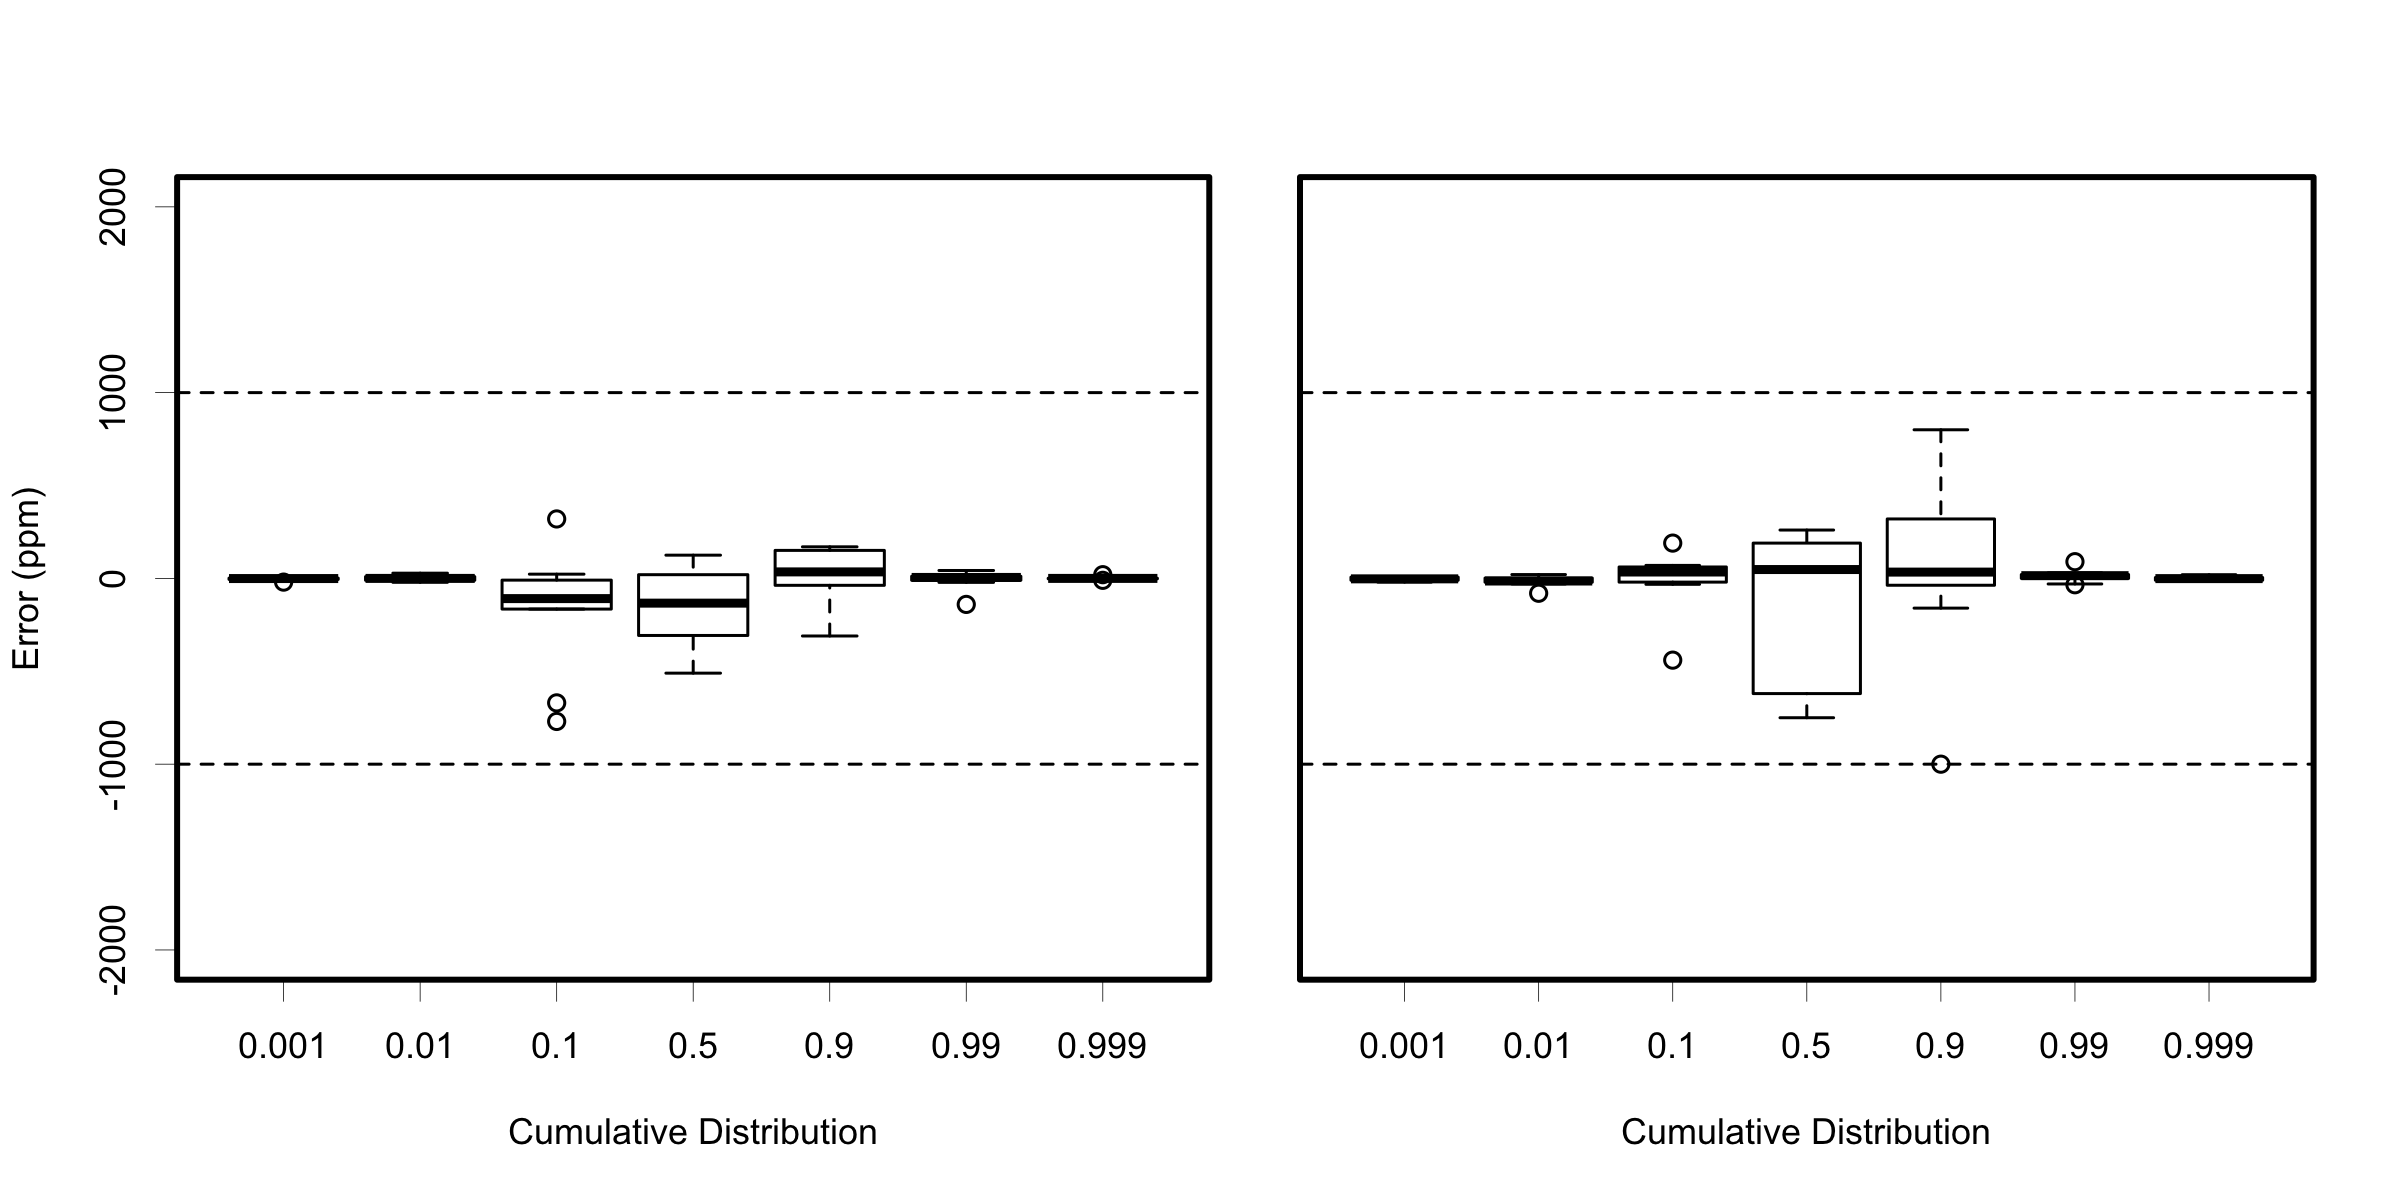
\includegraphics[width=6in]{error.png} 
   \caption{The absolute error of the estimate of the cumulative distribution function $q = \int_{-\infty}^x p(\alpha) \, d\alpha$ for the uniform distribution for 5 runs, each with 100,000 data points.  As can be seen, the error is dramatically decreased for very high or very low quantiles (to a few parts per million).  The precision setting used here, $1/\delta = 100$, would result in uniform error of 10,000 ppm without adaptive bin sizing and interpolation.}
   \label{fig:uniform-error}
\end{figure}

Obviously, with the relatively small numbers of samples such as are used in these experiments, the accuracy of $1-d$ clustering as an estimate of the quantiles of the underlying distribution cannot be better than the accuracy of these estimates computed using the sample data points themselves.  For the experiments here, the errors due to sampling completely dominate the errors introduced by $1-d$ sampling, especially at extreme values of $q$.  For much larger sample sets of billions of samples or more, this would be less true and the errors shown here would represent the accuracy of approximating the underlying distribution.

It should be noted that using a Q-Digest implemented with long integers is only able to store data with about 20 significant decimal figures.  This means that such a Q-digest would be inherently unable to even estimate the quantiles of the $\Gamma$ distribution tested here.
\subsection{Storing $1-d$ clusterings}
For the accuracy setting and test data used in these experiments, the $1-d$ clustering produced $820-860$ centroids.  The results of $1-d$ clustering can thus be stored by storing this many centroid means and weights.  If centroids are kept as double precision floating point numbers and counts kept as 4-byte integers, the $1-d$ clusterings resulting from from the accuracy tests described here would require about 10 kilobytes of storage for any of the distributions tested.

This size can be substantially decreased, however.  One simple option is to store differences between centroid means and to use a variable byte encoding such as zig-zag encoding to store the cluster size.  The differences between successive means are at least three orders of magnitude smaller than the means themselves so using single precision floating point to store these differences can allow the $1-d$ clusterings from the tests described here to be stored in about $4.6$ kilobytes while still regaining nearly 10 significant figures of accuracy in the means.  This is roughly equivalent to the precision possible with a Q-digest operating on 32 bit integers, but the dynamic range of $1-d$ clustering will be considerably higher and the accuracy is considerably better.
\subsection{Space/Accuracy Trade-off}
Not surprisingly, there is a strong trade-off between the size of the digest produced by $1-d$ clustering as controlled by the compression parameter $1/\delta$ and the accuracy which which quantiles are estimated.  Quantiles at $0.999$ and above or $0.001$ or below were estimated to within a small fraction of 1\% regardless of digest size.  Accurate estimates of the median require substantially larger digests.  Figure \ref{fig:accuracy-1} shows this basic trade-off.

The size of the resulting digest depends strongly on the compression parameter $1/\delta$ as shown in the left panel of Figure \ref{fig:accuracy-2}.  Size of the digest also grows roughly with the log of the number of samples observed, at least in the range of 10,000 to 10,000,000 samples shown in the right panel of Figure \ref{fig:accuracy-2}.

\begin{figure}[htb] %  figure placement: here, top, bottom, or page
   \centering
   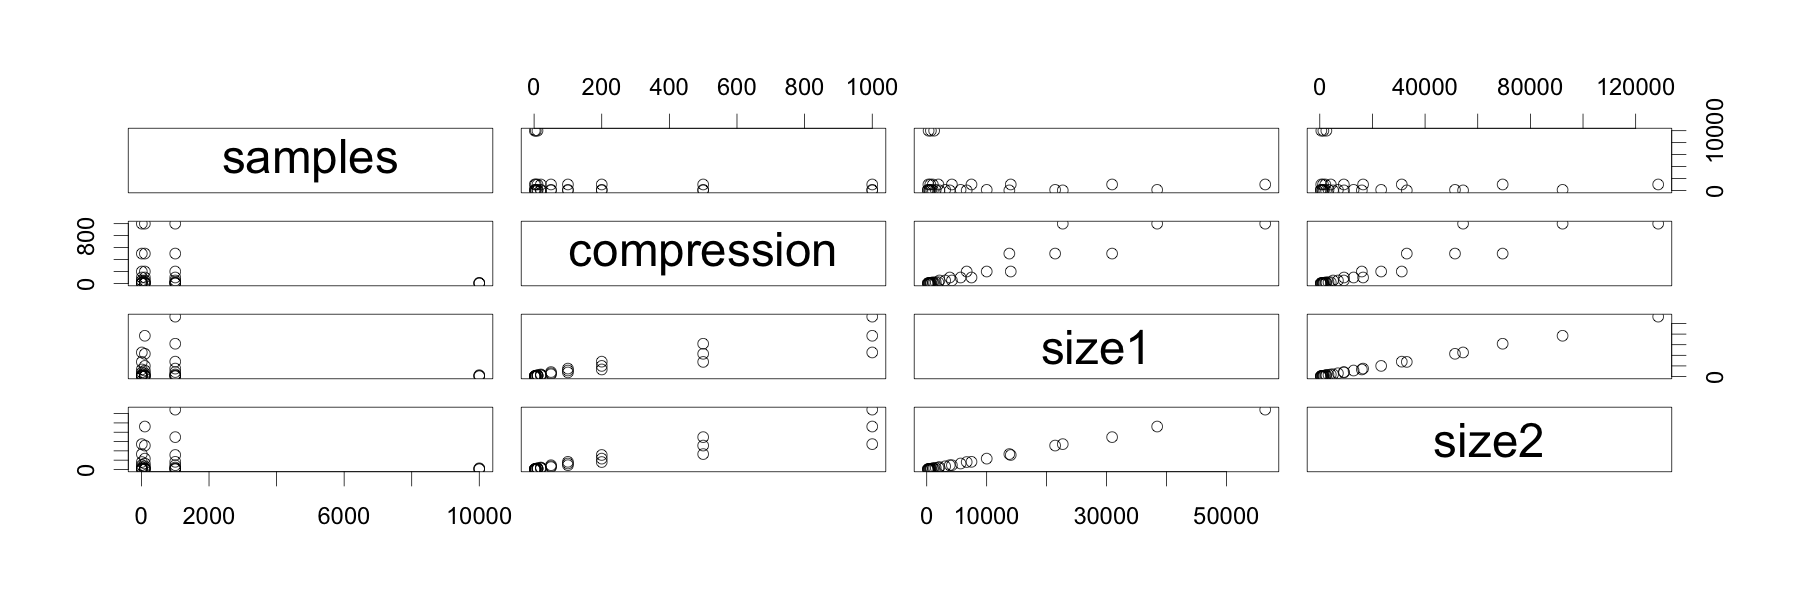
\includegraphics[width=6in]{accuracy-1.png} 
   \caption{Accuracy is good for extreme quantiles regardless of digest size.  For mid quantiles such as the median, moderate digest sizes suffice to get better than 1\% accuracy, but a digest must be 10kB or more to achieve 0.1\% accuracy.  All panels were computed using 40 runs with 100,000 samples.  Compression parameter ($1/\delta$) was varied from 2 to 1000 in order to vary the size of the resulting digest.  Sizes shown were encoded using 4 byte floating point delta encoding for the centroid means and variable byte length integer encoding.}
   \label{fig:accuracy-1}
\end{figure}
\begin{figure}[htb] %  figure placement: here, top, bottom, or page
   \centering
   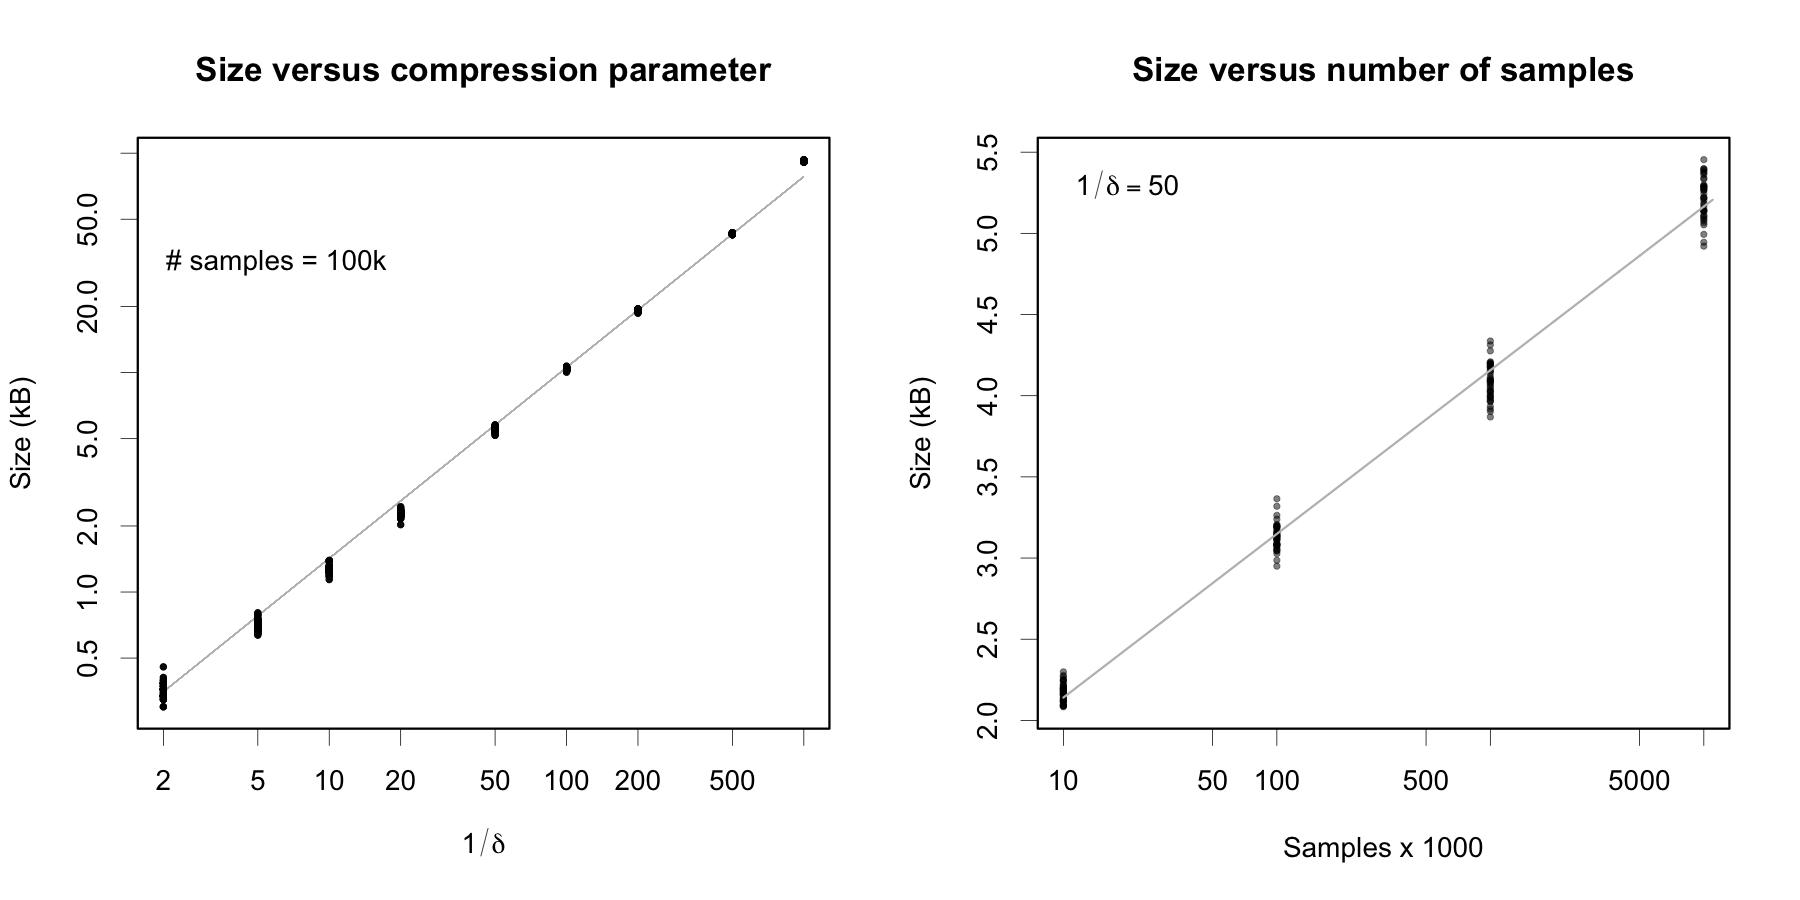
\includegraphics[width=6in]{accuracy-2.png} 
   \caption{Size of the digest scales sub-linearly with compression parameter ($\alpha \approx 0.9$) for fixed number of points.  Size scales approximately logarithmically with number of points for fixed compression parameter.  }
   \label{fig:accuracy-2}
\end{figure}

\subsection{Speed}
The current implementation has been primarily optimized for ease of development, not execution speed.  As it is, running on a single core of a 2.3 GHz Intel Core i5, it typically takes 2-3 microseconds to process each point
%\subsection{}
\bibliographystyle{alpha}
\bibliography{refs}{}

\end{document}  